\documentclass[../main.tex]{subfiles}

\begin{document}
	\section{Osservatore asintotico dello stato}
		$ \forall u(.) $, $ \forall \vec x(0^{-}) $, $ \forall \vec z(0^{-}) $, il sistema \textit{Osservatore} \'e definito \textbf{osservatore asintotico} se:
		\[
			\vec x(t) - \vec{\hat x}(t) \underset{t \rightarrow \infty}{\longrightarrow} 0
		\]
		Consideriamo i sistemi:
		\[
			S:
			\begin{cases}
				\vec{\dot x} = A \vec x + B \vec u\\
				\vec y = C \vec x
			\end{cases}
			\qquad
			Osservatore:
			\begin{cases}
				\vec{\dot z} = \hat A \vec z + \hat B \vec u + L \vec y\\
				\vec{\hat x} = \vec z
			\end{cases}
		\]
		
		\begin{figure}[H]
			\centering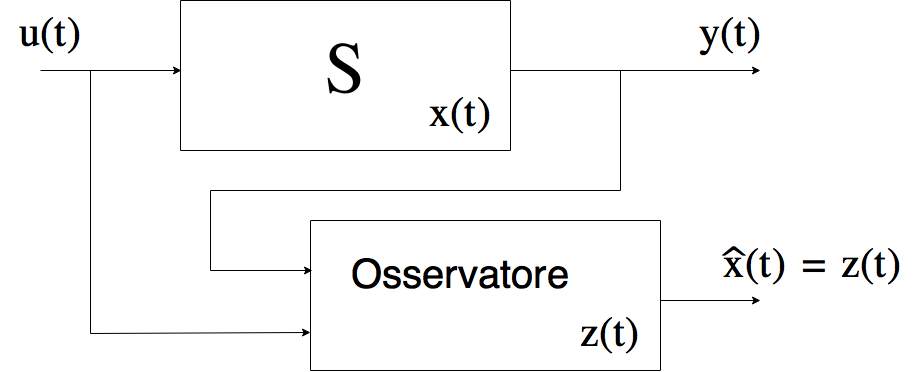
\includegraphics[width=.5\textwidth]{rappresentazione_sistema2/osservatore_asintotico}
		\end{figure}
		
		$ A, B, C $ note e $ x(0^{-}) $ incognito, dobbiamo determinare $ \hat A, \hat B, L $, tale che l'errore di stima $ \vec e(t) $:
		\[
			\vec e(t) \triangleq \vec x(t) - \vec{\hat x}(t) \underset{t \rightarrow \infty}{\longrightarrow} 0
		\]
		Studiamo come evolve l'errore:
		\begin{align*}
			\dot{\vec e}(t) &= \vec{\dot x}(t) - \dot{\vec{\hat{x}}}(t) = A \vec x(t) + B \vec u(t) - \left[ \hat A \vec z(t) + \hat B \vec u(t) + L \vec y(t) \right] =
			\\
			&= A \vec x(t) + B \vec u(t) - \hat{\vec z(t)} - \hat B \vec u(t) - LC \vec x(t) =
			\\\intertext{Scelgo $ \quad \hat B = B \qquad \hat A = A - LC $}
			&= (A-LC) \left[ \vec x(t) - \vec z(t) \right] = (A-LC) \vec e(t)			
		\end{align*}
		$ \vec e(t) $ evolve come lo stato di un sistema autonomo lineare con matrice $ (A-LC) $. Se $ L $ \'e tale che sia asintoticamente stabile (tutti gli autovalori a $ \Re < 0 $), si ottiene un osservatore asintotico.
		
		Avevamo visto (nella retroazione algebrica sullo stato), che se la coppia di matrici $ (A,B) $ \'e completamente controllabile, posso scegliere $ K $ tale che $ (A+BK) $ ha autovalori a piacere. Sfrutto la dualit\'a: se $ (C,A) $, \'e completamente osservabile, cio\'e il sistema $ S $ \'e completamente osservabile
		\[
			S:
			\begin{cases}
				\dot x = Ax + Bu\\
				y = Cx
			\end{cases}
		\]
		allora il suo sistema duale \'e completamente controllabile
		\[
			\dot w = A^T w + C^T v\\
			q = B^T w
		\]
		autovalori di $ (A^T + C^T K) $ sono assegnabili a piacere con la scelta di $ K $.\\
		Quindi se scegliamo $ L = -K^T $, allora $ (A-LC)^T = (A+K^TC)^T = A^T + C^TK $, cio\'e assegniamo $ L $ in modo che gli autovalori osservabili siano assegnabili a piacere in $ (A-LC) $.
		
		\begin{definition}
			Un sistema \'e \textit{detettabile} se e solo se gli autovalori osservabili sono tutti a $ \Re < 0 $. Quindi se un sistema \'e \textit{detettabile}, \'e possibile costruire un osservatore asintotico.
		\end{definition}
		
		\paragraph{Osservatore deterministico e non deterministico (stocastico)}
		La caratterizzazione tra un osservatore \textit{deterministico} e \textit{non deterministico} \'e del tutto generale. \'E evidente che la velocit\'a di convergenza dell'osservatore di stato pu\'o essere modificata agendo sulla matrice \textit{L}.\\
		Tipicamente viene associato a questo tipo di osservatore il nome di \textit{Osservatore di Luenberger} o di osservatore deterministico per distinguerlo dall'osservatore non deterministico detto \textit{Filtro di Kalman}.\\
		In realt\'a entrambi i tipi di osservatore hanno la medesima struttura e si differenziano solo per la scelta della matrice \textit{L}:
		\begin{itemize}
			\item nel caso deterministico la scelta \'e legata esclusivamente alla velocit\'a di convergenza della stima;
			\item nel caso non deterministico la scelta \'e influenzata dall'incertezza sulla misura di ${\vec {u}}(t)$ e ${\vec {y}}(t)$.
		\end{itemize}
		
	\subsection{Osservatore di Luenberger}
		\[
			\begin{cases}
				\dot{\vec z} = A \vec z + B \vec u + L (\vec y - C \vec z)\\
				\hat{\vec x} = \vec z
			\end{cases}
		\]
		Se $ L $ \'e tale che $ (A-LC) $ \'e asintoticamente stabile, allora si tratta di un osservatore asintotico.
		
		$ \hat{\vec y} = C \vec z = C \hat{\vec x} $ \'e una stima di $ \vec y $ se uso $ \vec z = \hat{\vec x} $, come stima di $ \vec x $:
		\[
			\begin{cases}
				\dot{\vec z} = A \vec z + B \vec u + L (\vec y - \hat{\vec y})\\
				\hat{\vec x} = \vec z\\
				\hat{\vec y} = C \vec z
			\end{cases}
		\]
		
	\subsection{Osservatore per controllo}
		\begin{figure}[H]
			\begin{subfigure}{0.5\textwidth}
				\[
					\begin{cases}
						\dot x = Ax + Bu\\
						y = Cx\\
						\dot z = Az + Bu + L(y-Cz)\\
						u = Kz + v
					\end{cases}
				\]
			\end{subfigure}
			\begin{subfigure}{0.5\textwidth}
				\centering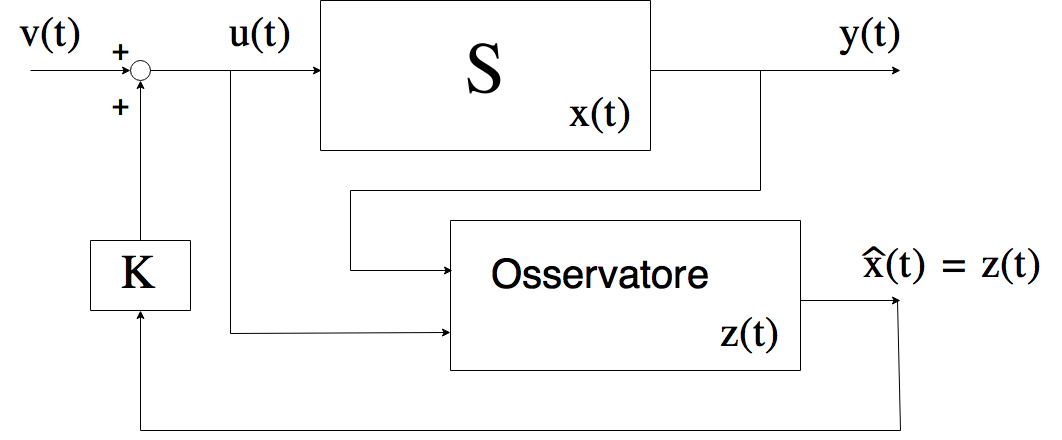
\includegraphics[width=1.1\textwidth]{rappresentazione_sistema2/osservatore_controllo}
			\end{subfigure}
		\end{figure}
		
		Cambio $ z $ con $ e = x-z $:
		\[
			\begin{cases}
				\dot x = Ax + B\left[ K(x-e)+v \right] = (A+BK) x - BKe + Bv\\
				\dot e = (A-LC) e\\
				y = Cx
			\end{cases}
		\]
		\[
			\begin{bmatrix}
				\dot x\\
				\dot e
			\end{bmatrix} = 
			\begin{bmatrix}
				A+BK & -BK\\
				0 & A-LC
			\end{bmatrix}
			\begin{bmatrix}
				x\\
				e
			\end{bmatrix} +
			\begin{bmatrix}
				B\\
				0
			\end{bmatrix} v
			\\
			y =
			\begin{bmatrix}
				C & 0
			\end{bmatrix}
			\begin{bmatrix}
				x\\
				e
			\end{bmatrix}
		\]
		\[
			\dot{\vec x} = \underbrace{(A+BK)x + Bv}_{\stackrel{come\ se\ facessi\ retroazione}{su\ x,\ non\ sulla\ stima}} - \underbrace{BKe}_{\stackrel{errore\ dovuto\ alla}{stima\ dello\ stato}}
		\]
		
		Se il sistema \'e completamente controllabile e osservabile, posso scegliere $ L $ tale che $ (A-LC) $ sia asintoticamente stabile (cio\'e che l'osservatore sia asintotico) e $ K $ tale che $ (A+BK) $ sia asintoticamente stabile (progetto di retroazione sullo stato).
		
		Quindi per i sistemi lineari vale il \textbf{principio di separazione}: osservatore e regolatore possono essere progettati separatamente.
		
		\begin{mdframed}[style=Exercise]
			\begin{Exercise}[title={Stabilizzazione di un sistema con osservatore}, difficulty=1]
				\[
					T(s) = \dfrac{1}{s^2}
				\]
				Abbiamo visto che si tratta di un sistema instabile e che non pu\'o essere stabilizzato con una retroazione algebrica sull'uscita. Proviamo quindi a stabilizzarlo con un osservatore asintotico.
				
				Realizziamo il sistema con la FCC:
				\[
					n = 2
					\qquad
					\begin{aligned}
						a_0 &= 0\\
						a_1 &= 0
					\end{aligned}
					\qquad
					\begin{aligned}
						b_0 &= 1\\
						b_1 &= 0\\
						b_2 &= 0
					\end{aligned}
				\]
				\[
					S:
					\begin{cases}
						\dot x =
						\begin{bmatrix}
							0 & 1\\
							0 & 0
						\end{bmatrix} x+
						\begin{bmatrix}
							0\\
							1
						\end{bmatrix} u
						\\[1em]
						y =
						\begin{bmatrix}
							1 & 0
						\end{bmatrix} x
					\end{cases}
				\]
				
				Progettiamo il regolatore:
				\[
					u = Kz + v \qquad\qquad K =
					\begin{bmatrix}
						K_1 & K_2
					\end{bmatrix}
				\]
				\[
					(A+BK) =
					\begin{bmatrix}
						0 & 1\\
						0 & 0
					\end{bmatrix} +
					\begin{bmatrix}
						0\\
						1
					\end{bmatrix}
					\begin{bmatrix}
						K_1 & K_2
					\end{bmatrix} =
					\begin{bmatrix}
						0 & 1\\
						K_1 & K_2
					\end{bmatrix}
				\]
				\[
					\varphi_{A+BK}(s) = det
					\begin{bmatrix}
						s & -1\\
						-K_1 & s-K_2
					\end{bmatrix} = s^2 - K_2s - K_1
				\]
				Se voglio entrambi gli autovalori in $ -1 $:
				\[
					\varphi_{A+BK}(s) = s^2 + 2s + 1 \quad\Leftrightarrow\quad K_1 = -1 \quad K_2 = -2
				\]
				
				Progettiamo l'osservatore:
				\[
					\begin{cases}
						\dot z = Az + Bu +L(y-Cz)\\
						\hat x = z
					\end{cases}
				\]
				$ L = \begin{bmatrix} l_1 \\ l_2 \end{bmatrix} $ tale che $ (A-LC) $ sia asintoticamente stabile.
				\[
					A-LC = 
					\begin{bmatrix}
						0 & 1\\
						0 & 0
					\end{bmatrix} -
					\begin{bmatrix}
						l_1\\
						l_2
					\end{bmatrix}
					\begin{bmatrix}
						1 & 0
					\end{bmatrix} = 
					\begin{bmatrix}
						-l_1 & 1\\
						-l_2 & 0
					\end{bmatrix}
				\]
				\[
					det\left[ sI - (A-LC) \right] = det 
					\begin{bmatrix}
						s+l_1 & -1\\
						l_2 & s
					\end{bmatrix} = s^2 + l_1 s + l_2
				\]
				\[
					\Rightarrow\quad l_1 = -2 \quad l_2 = 1
				\]
			\end{Exercise}
		\end{mdframed}
\end{document}